\documentclass{beamer}

\usepackage{hyperref}
\usepackage{bm}
\hypersetup{
  pdfinfo={
    CreationDate={D:20180702102722},
    ModDate={D:20180702102722},
  },
}

\AtBeginSection[]
{
  \begin{frame}
    \frametitle{Table of Contents}
    \tableofcontents[currentsection]
  \end{frame}
}

\usetheme{metropolis}
% Some configurations of metropolis theme
\metroset{block=fill}
\metroset{numbering=none}
% Set some custom colors for the beamer theme
\definecolor{DarkBlue}{HTML}{163a7a}
\definecolor{jr@medblue}{RGB}{103,169,207}
\definecolor{jr@green}{RGB}{77,175,74}
\definecolor{jr@darkred}{RGB}{153,0,0}
\setbeamercolor{frametitle}{bg=DarkBlue}
\setbeamercolor{progress bar}{fg=black}
\setbeamercolor{progress bar}{bg=black}
\setbeamercolor{background canvas}{bg=white}
% Use serif font for math
\usefonttheme[onlymath]{serif}
% Margins
\setbeamersize{text margin left=0.5cm,text margin right=0.5cm}
% Slide footer (optional)
\setbeamertemplate{footline}[text line]{%
\parbox{\linewidth}{\vspace*{-0.5cm}\small\hspace{11.15cm}%
\parbox{1cm}{\raggedleft\scriptsize\insertframenumber}}}
\setbeamertemplate{navigation symbols}{}

% lmss uses the computer modern tt font, better for URLs, etc.
\newcommand{\lmss}{\fontfamily{lmtt}\selectfont}
\newcommand{\eps}{\varepsilon}
\newcommand{\utri}{\mathcal{U}}

\title[Lagrange and B\'{e}zier]
  {High-order Solution Transfer between Curved Meshes and
  Ill-conditioned B\'{e}zier Curve Intersection}
\date{August 9, 2018}
\author{Danny Hermes}
\institute{{\lmss dhermes@berkeley.edu} \\
           UC Berkeley}
\titlegraphic{
  \vspace{5cm}\hfill
  
\includegraphics[height=1.5cm]{uc_berkeley_seal.pdf}
  \hspace{1.5cm}
}

\begin{document}

\maketitle

%%%%%%%%%%%%%%%%%%%%%%%%%%%%%%%%%%%%%%%%%%%%%%%%%%%%%%%%%%%%%%%%%%%%%%%%%%%%%%%%
%%%   OUTLINE   %%%%%%%%%%%%%%%%%%%%%%%%%%%%%%%%%%%%%%%%%%%%%%%%%%%%%%%%%%%%%%%%
%%%%%%%%%%%%%%%%%%%%%%%%%%%%%%%%%%%%%%%%%%%%%%%%%%%%%%%%%%%%%%%%%%%%%%%%%%%%%%%%
\begin{frame}
\centering
{\Large\bf Outline} \\
\rule{0.82\textwidth}{1pt} \\[20pt]
\begin{minipage}{0.78\textwidth}\raggedright
\begin{enumerate}
\item Introduction and motivation
\item Curved Elements
\item Solution Transfer
\item Compensated Evaluation
\item Modified Newton's for Intersection
\end{enumerate}
\end{minipage}
\end{frame}

%%%%%%%%%%%%%
%%% INTRO %%%
%%%%%%%%%%%%%

\begin{frame}
\centering
{\Large \bf Introduction and motivation}
\rule{0.82\textwidth}{1pt}
\end{frame}

\begin{frame}
\frametitle{Method of Characteristics}
\pause
Solve simple transport equation
\begin{equation*}
u_t + c u_x = 0, \quad u(x, 0) = u_0(x).
\end{equation*}
\pause
Divide physical domain
\begin{equation*}
x(t) = x_0 + ct
\end{equation*}
\pause
PDE becomes a (trivial) ODE
\begin{equation*}
\frac{d}{dt} u(x(t), t) = 0.
\end{equation*}
\end{frame}

\begin{frame}
\frametitle{Method of Characteristics}
\begin{center}
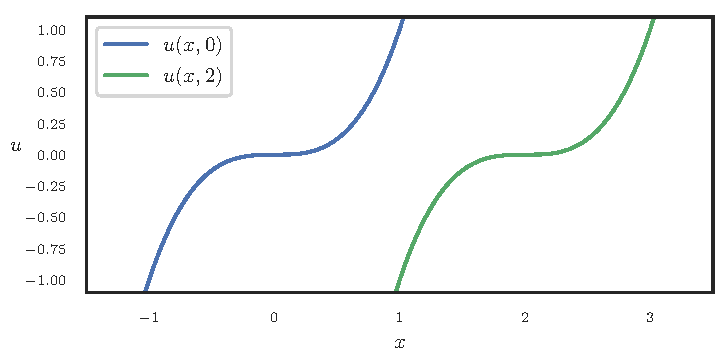
\includegraphics[width=0.95\textwidth]
                {../images/solution-transfer/simple_transport.pdf}
\end{center}
\end{frame}

\begin{frame}
\frametitle{Lagrangian Methods}
\begin{itemize}
\pause
\item Each point in physical domain is a \textbf{particle}
\pause
\item Carry value (e.g. heat, pressure, density) along characteristic curve
\pause
\item Transform PDE to family of ODEs
\end{itemize}
\end{frame}

\begin{frame}
\frametitle{Lagrangian Methods}
Add viscosity term to transport equation
\begin{equation*}
u_t + c u_x - \eps u_{xx} = 0.
\end{equation*}
\pause
Same characteristics used, \textbf{but} solution no
longer constant
\pause
\begin{equation*}
\frac{d}{dt} u(x(t), t) = \eps u_{xx}.
\end{equation*}
\end{frame}

\begin{frame}
\frametitle{Remeshing and Adaptivity}
\begin{itemize}
\item Problems caused by flow-based mesh changes
\begin{itemize}
\pause
\item Distortion
\pause
\item Tangling
\pause
\item Travel outside relevant physical domain
\end{itemize}
\pause
\item Adaptivity
\begin{itemize}
\pause
\item Dynamically focus computational effort
\pause
\item Resolve sensitive features
\end{itemize}
\end{itemize}
\end{frame}

\begin{frame}
\frametitle{Remeshing Example}
Consider
\begin{equation*}
u_t + \left[ \begin{array}{c} y^2 \\ 1 \end{array}\right] \cdot \nabla u +
  F\left(u, \nabla u\right) = 0
\end{equation*}
\pause
with cubic characteristics
\begin{equation*}
\left[ \begin{array}{c} x(t) \\ y(t) \end{array}\right] =
  \left[ \begin{array}{c} x_0 \\ y_0 \end{array}\right] +
  \frac{1}{3} \left[ \begin{array}{c} (y_0 + t)^3 - y_0^3 \\
  3t \end{array}\right].
\end{equation*}
\end{frame}

\begin{frame}
\frametitle{Remeshing Example}
\begin{center}
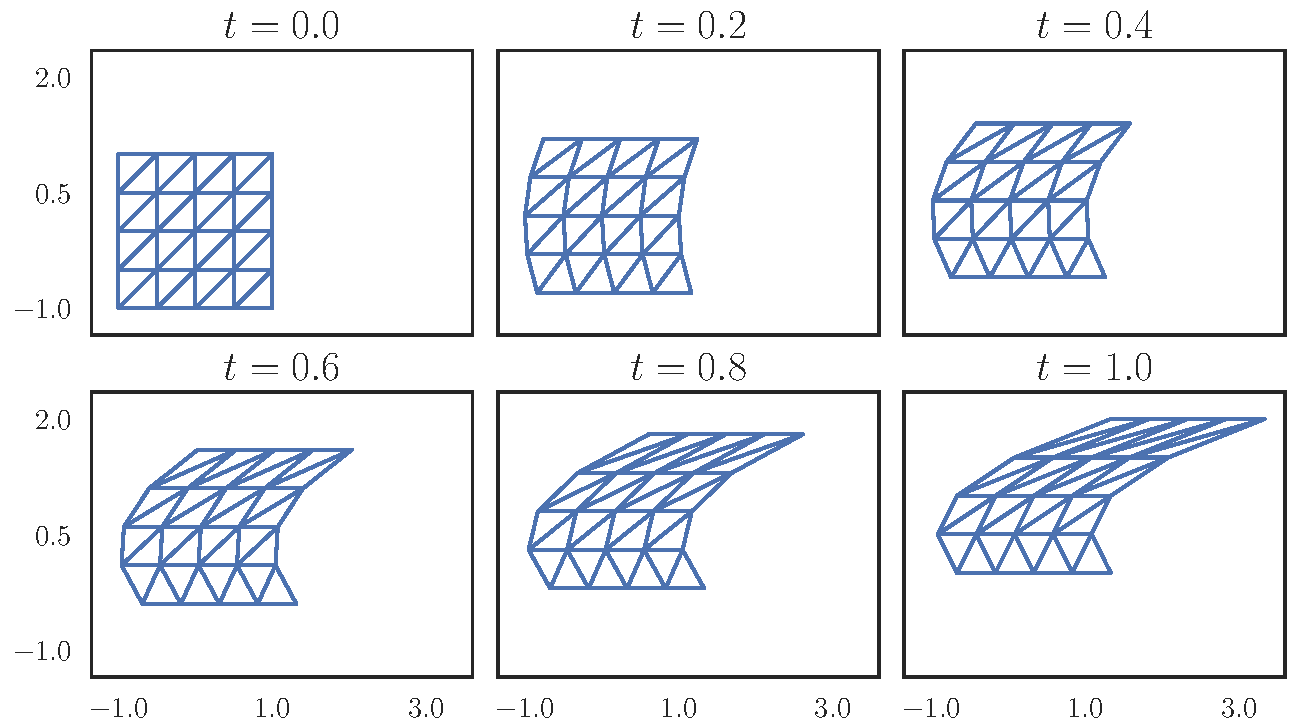
\includegraphics[width=0.95\textwidth]
                {../images/slides/mesh_distortion.pdf}
\end{center}
\end{frame}

\begin{frame}
\frametitle{Remeshing Example}
\begin{center}
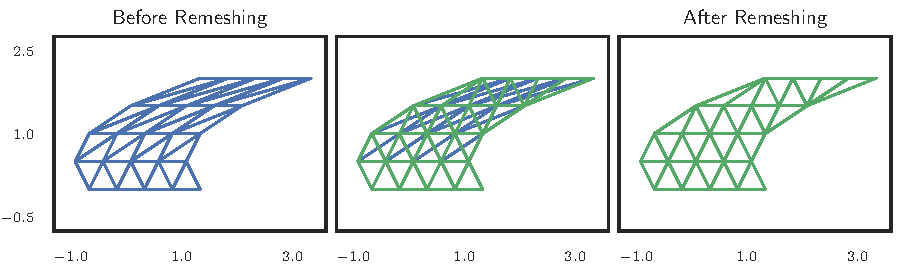
\includegraphics[width=0.95\textwidth]
                {../images/solution-transfer/distortion_remesh.pdf}
\end{center}
\end{frame}

\begin{frame}
\frametitle{Curved Meshes}
\only<1-5,7-11>{
\begin{itemize}
\item<1-5,7-11> Benefits
\begin{itemize}
\item<2-5,7-11> High-order shape functions, highly accurate solutions
\item<3-5,7-11> Low dissipation and dispersion error
\item<4-5,7-11> Greater geometric flexibility
\item<5,7-11> Fewer elements
\end{itemize}
\item<8-11> Drawbacks
\begin{itemize}
\item<9-11> Harder to implement
\item<10-11> Loss of accuracy in high degree (e.g. Runge's phenomenon)
\item<11> More challenging geometry
\end{itemize}
\end{itemize}
}
%%
\begin{center}
\includegraphics<6>[width=0.95\textwidth]
                   {../images/solution-transfer/main_figure27.pdf}
\includegraphics<12>[width=0.95\textwidth]
                    {../images/slides/not_convex.pdf}
\includegraphics<13>[width=0.95\textwidth]
                    {../images/slides/split_intersection.pdf}
\end{center}
\end{frame}

\begin{frame}
\frametitle{Curved Elements}
\begin{itemize}
\item Necessary for High-order
\pause
\item With non-linear shape functions (i.e. not straight sided), non-vertex
nodes used
\pause
\item Lagrangian method must either curve mesh or information about
flow of geometry will be lost
\end{itemize}
\end{frame}

\begin{frame}
\frametitle{Curved Elements: Necessary for High-order}
%% H/T: https://stackoverflow.com/a/4684091/1068170
\begin{center}
\includegraphics<1>[width=0.95\textwidth]
                   {../images/slides/element_distortion1.pdf}
\includegraphics<2>[width=0.95\textwidth]
                   {../images/slides/element_distortion2.pdf}
\includegraphics<3>[width=0.95\textwidth]
                   {../images/slides/element_distortion3.pdf}
\end{center}
\end{frame}

%%%%%%%%%%%%%%%%%%%%%%%
%%% CURVED ELEMENTS %%%
%%%%%%%%%%%%%%%%%%%%%%%

\begin{frame}
\centering
{\Large \bf Curved Elements}
\rule{0.82\textwidth}{1pt}
\end{frame}

\begin{frame}
\frametitle{B\'{e}zier Triangles}
\begin{itemize}
\item Image \(\mathcal{T} = b\left(\utri\right)\) of reference triangle
  under polynomial map \(b(s, t)\)
\pause
\item Barycentric
  coordinates \(\lambda_1 = 1 - s - t, \lambda_2 = s, \lambda_3 = t\)
\pause
\item Bernstein basis via trinomial expansion:
\begin{equation*}
1 = \left(\lambda_1 + \lambda_2 + \lambda_3\right)^n
\end{equation*}
\pause
\vspace*{-0.9cm}
\item Convex combination of control points
\begin{equation*}
b(s, t) = \sum_{\substack{i + j + k = n \\ i, j, k \geq 0}}
  \binom{n}{i, j, k} \lambda_1^i \lambda_2^j \lambda_3^k \;
  \bm{p}_{i, j, k}
\end{equation*}
\end{itemize}
\end{frame}

\begin{frame}
\frametitle{B\'{e}zier Triangles}
\begin{center}
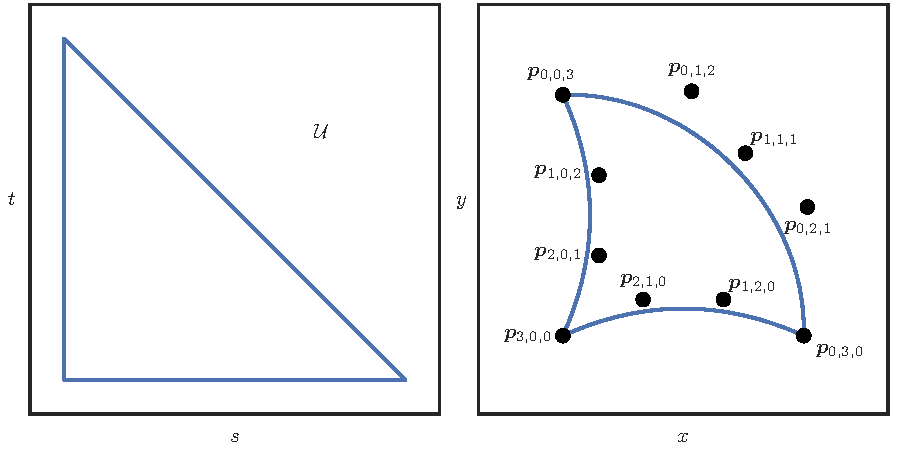
\includegraphics[width=0.95\textwidth]
                {../images/slides/main_figure31.pdf}
\end{center}
\end{frame}

\begin{frame}
\frametitle{B\'{e}zier Triangles}
\only<1-3,5-7>{
\begin{itemize}
\item<1-3,5-7> \(b(s, t)\) can be defined by data other than control net
\item<2-3,5-7> Regular grid in \(\utri\), \(\bm{u}_{i, j, k} =
  \left(\frac{j}{n}, \frac{k}{n}\right)\)
\item<3,5-7> \(b\left(\bm{u}_{i, j, k}\right) = \bm{n}_{i, j, k}\); refer to
  \(\bm{n}_{i, j, k}\) as \textbf{standard nodes}
\item<6-7> For example, taking \(\bm{n}_{i, j, k} = \delta_{(i, j, k) \;
  (i_0, j_0, k_0)}\) gives degree \(n\) shape functions on \(\utri\)
\item<7> Conversion between \(\bm{n}_{i, j, k}\) and \(\bm{p}_{i, j, k}\)
  has condition number exponential in \(n\)
\end{itemize}
}
%%
\begin{center}
\includegraphics<4>[width=0.95\textwidth]
                  {../images/preliminaries/main_figure01.pdf}
\end{center}
\end{frame}

\begin{frame}
\frametitle{Valid Element}
\begin{itemize}
\item Element \(\mathcal{T}\) is \textbf{valid} if diffeomorphic to
  \(\utri\)
\pause
\item \(b(s, t)\) bijective, i.e. Jacobian \(Db\) is everywhere invertible
\pause
\item \(\det(Db)\) positive, preserves orientation
\end{itemize}
\end{frame}

\begin{frame}
\frametitle{Inverted Element}
Consider element given by map
\begin{equation*}
b(s, t) = \lambda_1^2 \left[ \begin{array}{c} 1 \\ 0 \end{array}\right] +
\lambda_2^2 \left[ \begin{array}{c} 1 \\ 1 \end{array}\right] +
\lambda_3^2 \left[ \begin{array}{c} 0 \\ 1 \end{array}\right]
\end{equation*}
\end{frame}

\begin{frame}
\frametitle{Inverted Element}
\begin{center}
\includegraphics<1>[width=0.625\textwidth]{../images/slides/boundary_leak1.pdf}
\includegraphics<2>[width=0.625\textwidth]{../images/slides/boundary_leak2.pdf}
\includegraphics<3>[width=0.625\textwidth]{../images/slides/boundary_leak3.pdf}
\includegraphics<4>[width=0.625\textwidth]{../images/slides/boundary_leak4.pdf}
\includegraphics<5>[width=0.625\textwidth]{../images/slides/boundary_leak5.pdf}
\includegraphics<6>[width=0.625\textwidth]{../images/slides/boundary_leak6.pdf}
\end{center}
\end{frame}

\begin{frame}
\frametitle{Inverted Element}
\begin{center}
\includegraphics<1>[width=0.95\textwidth]
                   {../images/slides/inverted_element1.pdf}
\includegraphics<2>[width=0.95\textwidth]
                   {../images/slides/inverted_element2.pdf}
\includegraphics<3>[width=0.95\textwidth]
                   {../images/slides/inverted_element3.pdf}
\end{center}
\end{frame}

\begin{frame}
\frametitle{Shape Functions}
\only<1-2,5-8>{
\begin{itemize}
\item<1-2,5-8> Based on \(\bm{u}_{\bm{\alpha}} \in \utri\) or
  \(\bm{n}_{\bm{\alpha}} \in \mathbf{R}^2\)
  (\(\bm{\alpha}\) is a multi-index)
\item<2,5-8> \textbf{Pre-Image Basis}: \(\phi_{\bm{\alpha}}\left(
  \bm{n}_{\bm{\beta}}\right) = \widehat{\phi}_{\bm{\alpha}}\left(
  \bm{u}_{\bm{\beta}}\right) = \widehat{\phi}_{\bm{\alpha}}\left(b^{-1}\left(
  \bm{n}_{\bm{\beta}}\right)\right)\)
\item<6-8> \textbf{Global Coordinates Basis}: \(\phi_{\bm{\alpha}}\left(
  \bm{n}_{\bm{\beta}}\right) = \delta_{\bm{\alpha} \bm{\beta}}\)
\item<7-8> Element is \textbf{isoparametric} when numerical solution
  expressed in span of shape functions
\item<8> \(\operatorname{supp}(\phi) = \mathcal{T}\)
\end{itemize}
}
%%
\begin{center}
\includegraphics<3>{tikz_shape_fns1.pdf}
\includegraphics<4>{tikz_shape_fns2.pdf}
\end{center}
\end{frame}

%%%%%%%%%%%%%%%%%%%%%%%%%
%%% SOLUTION TRANSFER %%%
%%%%%%%%%%%%%%%%%%%%%%%%%

\begin{frame}
\centering
{\Large \bf Solution Transfer}
\rule{0.82\textwidth}{1pt}
\end{frame}

\begin{frame}
\frametitle{Galerkin Projection}
\begin{itemize}
\item \textbf{Given}:
\begin{itemize}
\pause
\item Donor mesh \(\mathcal{M}_D\) and target mesh \(\mathcal{M}_T\)
\pause
\item Shape function bases \(\phi_D^{(j)}\) and \(\phi_T^{(j)}\)
\pause
\item Known discrete field \(\bm{q}_D = \sum_j d_j \phi_D^{(j)}\)
\end{itemize}
\pause
\item \textbf{Want}: \(L_2\)-optimal interpolant
\(\bm{q}_T = \sum_j t_j \phi_T^{(j)}\):
\begin{equation*}
\left \lVert \bm{q}_T - \bm{q}_D \right \rVert_2 =
\min_{\bm{q} \in \mathcal{V}_T}
\left \lVert \bm{q} - \bm{q}_D \right \rVert_2
\end{equation*}
\end{itemize}
\end{frame}

\begin{frame}
\frametitle{Galerkin Projection}
Differentiating w.r.t. each \(t_j\) in
\(\bm{q}_T = \sum_j t_j \phi_T^{(j)}\) gives \textbf{weak form}
\begin{equation*}
\int_{\Omega} \bm{q}_D \phi_T^{(j)} \, dV =
  \int_{\Omega} \bm{q}_T \phi_T^{(j)} \, dV, \qquad \text{for all } j.
\end{equation*}
\pause
If \(\left(\bm{x} \mapsto 1\right) \in \mathcal{V}_T\), then \(\bm{q}_T\)
is globally \textbf{conservative}
\begin{equation*}
\int_{\Omega} \bm{q}_D \, dV =
  \int_{\Omega} \bm{q}_T \, dV.
\end{equation*}
\end{frame}

\begin{frame}
\frametitle{Linear System}
Weak form gives rise to a linear system in coefficients
\(\bm{d}\) and \(\bm{t}\):
\pause
\begin{equation*}
M_T \bm{t} = M_{TD} \bm{d}.
\end{equation*}
\pause
\(M_T\) is (symmetric) mass matrix for target mesh
\begin{equation*}
\left(M_T\right)_{ij} = \int_{\Omega} \phi_T^{(i)} \phi_T^{(j)} \, dV.
\end{equation*}
\end{frame}

\begin{frame}
\frametitle{Linear System}
Each shape function \(\phi\) has
\(\operatorname{supp}(\phi) = \mathcal{T}\) for some (curved)
element, hence \(M_T\) is block diagonal in DG,
sparse but globally coupled in CG.
\end{frame}

%%%%%%%%%%%%%%%%%%%%%%%%%%%%%%
%%% COMPENSATED EVALUATION %%%
%%%%%%%%%%%%%%%%%%%%%%%%%%%%%%

\begin{frame}
\centering
{\Large \bf Compensated Evaluation}
\rule{0.82\textwidth}{1pt}
\end{frame}

%%%%%%%%%%%%%%%%%%%%%%%%%%%%%%%%%%%%%%%%%%
%%% MODIFIED NEWTON'S FOR INTERSECTION %%%
%%%%%%%%%%%%%%%%%%%%%%%%%%%%%%%%%%%%%%%%%%

\begin{frame}
\centering
{\Large \bf Modified Newton's for Intersection}
\rule{0.82\textwidth}{1pt}
\end{frame}

\end{document}
